\documentclass[a4paper, 12pt]{article}

\usepackage[utf8]{inputenc}
\usepackage[T2A]{fontenc}
\usepackage[english,russian]{babel}

\usepackage{amsmath,amssymb,amsthm}

\usepackage{biblatex}
\usepackage{hyperref}

\usepackage[dvipsnames]{xcolor}

\usepackage{graphicx}
\usepackage{tikz-cd}
\usepackage[a4paper,hmargin=2.5cm,vmargin=2.5cm]{geometry}

\usepackage{enumitem}


\addbibresource{refs.bib}


\newtheorem*{theorem}{Теорема}
\newtheorem{definition}{Определение}
\newtheorem*{lemma}{Лемма}


\begin{document}


%%
%% Title page
%%

\begin{center}
{\scshape Федеральное государственное автономное\\
образовательное учреждение высшего образования\\
<<Национальный исследовательский университет\\
<<Высшая школа экономики>>\\[1ex]
Факультет математики\par}

\par\vfill

\textbf{\large Дьяконов Фёдор Юрьевич}

\vspace{1.5cm}

{\Large\bfseries
Гомологии трёхмерных многообразий
\par}

\vspace{1.5cm}

Курсовая работа студента 1 курса\\[1ex]
образовательной программы бакалавриата <<Математика>>
\par\vfill
\noindent\hspace{0.52\textwidth}\parbox[t]{0.48\textwidth}{%
Научный руководитель:\\[3pt]
Рябичев Андрей Дмитриевич\\[2ex]
}%
\par\vfill
Москва 2023
\end{center}
\thispagestyle{empty}

\pagebreak

\begin{abstract}
    В этой работе освещается построение гомологической 3-сферы. Для этого мы предварительно упрощаем задачу до построения 3-многообразия с совершенной фундаментальной группой. Далее при помощи вычислительных методов мы находим сбалансированное задание некоторой такой группы образующими и соотношениями, что позволяет сконструировать по нему многообразие как разбиение Хегора.
\end{abstract}


\section{Предварительные алгебраические утверждения}

    Чтобы построить искомое 3-многообразие, обладающее теми же гомологиями, что и у $\mathbb{S}^3$, мы предварительно введем несколько теорем, которые позволят нам свести эту задачу к поиску 3-многообразия, фундаментальная группа которого совершенна, то есть обладает тривиальной абелианизацией.

    \subsection{Теорема Гуревича}

        \begin{theorem}
            Для линейно связного топологического пространства $X$ верно, что
                 \begin{equation*} H_1(X, \mathbb{Z}) \cong \pi_1(X)_{ab}, \end{equation*}
            где последнее обозначает абелианизацию фундаментальной группы $X$.
        \end{theorem}

        \begin{proof}
            См., например, доказательство в \cite[Chapter~2,~Section~2.A]{Hatcher2001-hm}.
        \end{proof}

    \subsection{Двойственность Пуанкаре}

        \begin{theorem}
            Для связного ориентируемого $n$-многообразия $M$ существует изоморфизм между его группами когомологий и гомологий:
                \[ \begin{tikzcd}
                     H^k(M, \mathbb{Z}) \arrow{r}[label]{\sim} & H_{n - k}(M, \mathbb{Z}) 
                \end{tikzcd} \]
        \end{theorem}

        \begin{proof}
            См. доказательство в \cite[Chapter~3,~Section~3.3]{Hatcher2001-hm}.
        \end{proof}

    \subsection{Теорема об универсальных коэффициентах}

        \begin{theorem}
            Для цепного комплекса свободных абелевых групп $C_\bullet$, группы гомологий (над $\mathbb{Z}$) которого мы обозначим за $H_n$, существует и расщепляется точная последовательность
                \[ \begin{tikzcd}
                    0 \arrow{r} & \textnormal{Ext}(H_{n - 1}(C_\bullet), \mathbb{Z}) \arrow{r} & H^n(C_\bullet) \arrow{r} & \textnormal{Hom}(H_n(C_\bullet), \mathbb{Z}) \arrow{r} & 0 
                \end{tikzcd} \]
            \end{theorem}

        \begin{proof}
            См. доказательство в \cite[Chapter~3,~Section~3.1]{Hatcher2001-hm}.
        \end{proof}

    % \pagebreak
    \subsection{Следствия}

        Для линейно связного ориентируемого замкнутого 3-многообразия $M$ его нулевые гомологии и когомологии равны $\mathbb{Z}$, и также $H^3(M) = H_3(M) = \mathbb{Z}$. Предположим, что \begin{equation*} \pi_1(M)_{ab} = H_1(M) = 0. \end{equation*} Докажем тогда, что его первые когомологии тоже ноль, запишем формулу универсальных коэффициентов:


            \[ \begin{tikzcd}
                0 & {\textnormal{Ext}(H_0(M), \mathbb{Z}) } \arrow[draw=none]{d}[marking]{\cong} & {H^1(M)} & {\textnormal{Hom}(H_1(M), \mathbb{Z})) } \arrow[draw=none]{d}[marking]{\cong} & 0 \\
                & {\textnormal{Ext}(0, \mathbb{Z}) = 0} & & \textnormal{Hom}(0, \mathbb{Z}) = 0,
                \arrow[from=1-1, to=1-2]
                \arrow[from=1-2, to=1-3]
                \arrow[from=1-3, to=1-4]
                \arrow[from=1-4, to=1-5]
                % \arrow[from=1-2, to=2-3]
            \end{tikzcd} \]
        то есть мы получим, что $H^1(M) = 0 \oplus 0 = 0$. 
    
        Отсюда при применении двойственности Пуанкаре сразу следует, что \[H_2(M) = H_1(M) = 0.\]
    
        Следовательно, группы гомологий и когомологий связного ориентируемого и замкнутого 3-многообразия $M$ совпадают с такими у 3-сферы, когда $H_1(M) = 0$, то есть когда $\pi_1(M)_{ab} = 0$, и именно в таком виде мы и будем искать это многообразие. 
    

\section{Некоторые конструкции из маломерной топологии}

    \subsection{Определения}
    
        В интересах построения трехмерных многообразий мы воспользуемся инструментами, подробно описанными в \cite[Глава 4]{1997-hj}, здесь же мы кратко опишем основные определения. 

        \begin{definition}
            \colorbox{lime}{Разбиением Хегора} ориентируемого трехмерного многообразия $M$ называют его представление в виде объединения двух тел с ручками $M_1^3$ и $M_2^3$ с общей границей $\partial M_1^3 = \partial M_2^3$, отождествленной по некоторому гомеоморфизму.
        \end{definition}

        \begin{definition}
            \colorbox{lime}{Диаграммой Хегора} называют систему замкнутых ориентированных простых кривых $u_1, \dots, u_g$ и $v_1, \dots, v_g$ на сфере с $g$ ручками, которые удовлетворяют следующим условиям: 

            \begin{minipage}[t]{\linewidth}
                \begin{enumerate}[label=(\roman*)]
                    \item кривые $u_i$ попарно не пересекаются и дополнение к их объединению связно;
                    \item кривые $v_i$ попарно не пересекаются и дополнение к их объединению связно.
                \end{enumerate}
             \end{minipage}
        
        \end{definition}

        \begin{theorem}
            Всякая диаграмма Хегора задает разбиение Хегора, причем получаемый гомеоморфизм разбиения переводит две системы кривых диаграммы друг в друга.
        \end{theorem}

        \begin{proof}
            См. доказательство в \cite[Глава 4, \S 10.3]{1997-hj}
        \end{proof}

    \subsection{Фундаментальная группа 3-многообразия \\ с данным разбиением Хегора}

        Чтобы контролировать алгебраические инварианты искомого многообразия, мы воспользуемся следующей теоремой:

        \begin{theorem} \label{fgroup}
            Пусть $M$ задано разбиением Хегора на два тела с ручками рода $g$. Тогда у фундаментальной группы $M$ существует сбалансированное копредставление с $g$ образующими и $g$ соотношениями.
        \end{theorem}

        \begin{proof}
            Предположим, что $M$ разбито на тела $M_1$ и $M_2$ по гомеоморфизму $f: \partial M_1 \rightarrow \partial M_2$. Рассмотрим $g$ меридианов $w_1, \dots, w_g$ на $M_1$, которые ограничивают диски $D_1, \dots, D_g$ внутри тела.

            Так как $M \cong M_1 \cup_f M_2$, а дополнение к $\bigsqcup_{i = 1}^{g} D_i$ во внутренности $M_1$ гомеоморфно трёхмерному диску, то 

            \[\pi_1(M) \cong \pi_1( ~ (\bigsqcup_{i = 1}^{g} D_i) ~ \cup_f M_2),\] 
            поскольку фундаментальная группа клеточного комплекса зависит только от его 2-скелета.
            
            В свою очередь, $M_2$ гомотопически ретрагируется на букет $g$ окружностей, назовём эту ретракцию $\rho$. Тогда


            \[\pi_1(M) \cong \pi_1( ~ (\bigsqcup_{i = 1}^{g} D_i) ~ \cup_{\rho \circ f} \bigwedge_{j = 1}^{g} \mathbb{S}^1) \]

            Где справа написано клеточное разбиение пространства с одной 0-клеткой, $g$ 1-клетками и $g$ 2-клетками, приклеенными по характеристическим отображениям, которые получаются ограничением $\rho \circ f$ на $w_i$, что и дает нам искомое копредставление. 
            
        \end{proof}
        Более того, если это разбиение Хегора было получено из диаграммы Хегора, в которой первый набор кривых был выбран как меридианы на $M_1$, то соотношения в полученной группе будут определены образами второго набора кривых при ретракции, чем мы и воспользуемся далее.

\section{Обзор использованных вычислительных методов}     
    Чтобы найти совершенную группу и некоторое ее сбалансированное копредставление, мы выбрали подход перебора таких копредставлений и затем проверки свойств полученных групп.

    Хотя проблема доказательства тривиальности группы по ее копредставлению алгебраически неразрешима, проверка тривиальности ее абелианизации весьма проста в силу следующего утверждения:

    \begin{lemma}
        Пусть группа $G$ задана копредставлением $\langle e_1, e_2, \dots e_n \mid w_1, w_2, \dots, w_n \rangle$ c $n$ образующими и $n$ соотношениями, длина которых (то есть сокращенная запись из символов $e_i$ и $e_i^{-1}$) не превосходит $l$.
        
        Тогда тривиальность ее абелианизации $G_{ab}$ можно установить за временную сложность $O(n l + f(n))$, где $f(n)$ обозначает асимптотику работы алгоритма поиска определителя квадратной матрицы размера $n$, то есть, например, $O(n^3)$.
    \end{lemma}

    \begin{proof}
        В абелианизации $G$ соотношения в изначальной группе сводятся к словам $w^{ab}_i$ вида $e_1^{\alpha_{i, 1}} e_2^{\alpha_{i, 2}} \dots e_n^{\alpha_{i, n}}$. Итоговая группа тогда изоморфна фактору $\mathbb{Z}^n$ по целочисленной решетке, порожденной векторами, полученными из $w^{ab}_i$.

        В силу теоремы о существовании нормальной формы Смита у матрицы над кольцом главных идеалов, фактор по этой решетке, заданной матрицей $A = \alpha_{i, j}$ изоморфен фактору по решетке, порожденной диагональной матрицей $D$, где $D = P A Q$, причем матрицы $P$ и $Q$ обратимы.

        Такой фактор тривиален тогда и только тогда, когда все диагональные элементы $D$ равны $\pm 1$, что в силу целочисленности матрицы равностильно тому, что $\det D = \det A = \pm 1$.

        Тогда искомый алгоритм можно реализовать, сначала вычислив элементы матрицы $A$, что занимает $O(n l)$ времени, и затем посчитав определитель $A$ за сложность $O(f(n))$.
    \end{proof}

    Чтобы упростить реализацию соотношений в полученном копредставлении как системы простых кривых на сфере с $g$ ручками, мы зафиксировали $g = 2$, то есть перебор велся по двухгенераторным сбалансированным копредставлениям. При эффективной генерации копредставлений это значило, что матрица $A$ в лемме выше сводилась к четырем значениям, которые можно вычислить непосредственно в процессе генерации, а вычисление выше означает лишь подсчет определителя матрицы 2 на 2.

    Таким образом, в процессе перебора мы за константное время узнаем, тривиальна ли абелианизация группы. Однако для каждого из них оставалась возможность того, что и сама группа тривиальна, и, значит, не подходит нам.

    Чтобы исключить такие копредставления, мы затем пользовались алгоритмом Тодда — Коксетера перечисления смежных классов группы, заданной копредставлением, по некоторой ее подгруппе (см., например, \cite[Chapter 5]{Holt2005}), который, если группа имеет достаточно малый порядок и нетривиальна, дает нам этот результат за фиксированное число операций.

    Если же за определенное число операций (то есть для достаточно малой таблицы смежных классов) мы не получали положительного результата, или получали, что группа тривиальна, мы останавливали алгоритм и переходили к следующему копредставлению.

    Эти вычисления производились при помощи программы на языке программирования Julia \cite{Julia-2017} с интерфейсом к системе компьютерной алгебры GAP \cite{GAP4}, в которой реализован алгоритм Тодда — Коксетера. Исходный код и результаты вычислений предоставлены в репозитории \cite{Dyakonov2023}.
    

\section{Результаты}
    Мы перебрали все сбалансированные двухгенераторные копредставления групп, в которых длина соотношений (выраженная в терминах образующих и их обратных) хотя бы 3 и не превосходит 7.

    За время порядка десяти минут на одном персональном компьютере это дало порядка 600 различных (с точностью до естественных симметрий) копредставлений, которые задают нетривиальную конечную совершенную группу. Все их них при ближайшем рассмотрении оказались изоморфны $\textnormal{SL}_2(\mathbb{F}_5)$.

    Мы выбрали одно из них, а именно $G = \langle a, b \mid a b a^{-4} b, (b a)^2 b^{-3} \rangle$, и реализовали соотношения в нем как пунктированные кривые на сфере с двумя ручками, которые при ретракции на букет двух окружностей (стягивающей отмеченные точки на кривых в отмеченную точку букета) дадут эти элементы в фундаментальной группе. 
    
    При этом порождающая $a$ в букете соответствует кривой, обходящей один раз вокруг правой (см. рисунок) окружности, порождающая $b$ соответствует кривой, обходящей один раз вокруг левой окружности: 

    \vspace{1cm}

    \begin{figure}[h] 
        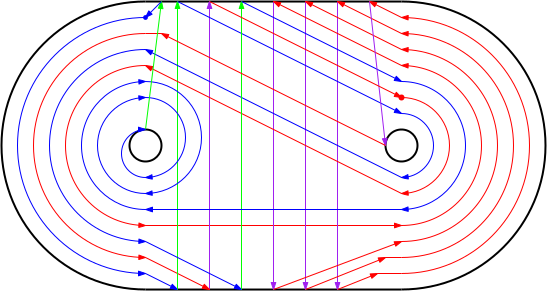
\includegraphics[width=\textwidth]{diagram}
        \caption{Реализация соотношений как системы попарно непересекающихся простых кривых. Здесь первое соотношение соответствует кривой, обозначенной красным и фиолетовым цветом, где красная часть находится на стороне поверхности, обращенной к наблюдателю, а фиолетовая на обратной. Аналогично соответственно синим и зеленым цветом обозначена вторая кривая. При этом кривые попарно не пересекаются, а дополнение к ним линейно связно.}
    \end{figure}

    Полученная мультикривая удовлетворяет требованиям для одного из набора кривых диаграммы Хегора, и если мы дополним ее вторым набором, состоящим из меридианов на сфере с двумя ручками, то в силу теоремы из раздела \ref{fgroup} фундаментальная группа полученного 3-многообразия будет иметь копредставление $G$, то есть будет изоморфна $\textnormal{SL}_2(\mathbb{F}_5)$ и совершенна.

    Что и дает нам искомое построение.

\section{Дальшейшая работа}
    Остается открытым вопрос построения гомологических 3-сфер с фундаментальными группами, не изоморфными $\textnormal{SL}_2(\mathbb{F}_5)$, что может быть достигнуто при дальшейшей оптимизации алгоритма перебора копредставлений, а также проведении большего объема вычислений. Это не было реализовано в этой работе в силу ограничений во времени, а также нашего фокуса на том, чтобы построить хоть один пример гомологической сферы без претензии на исчерпывающую их классификацию.

    Также интерес представляет общий вопрос реализуемости соотношений в полученных копредставлениях как мультикривых на сферах с $g$ ручками. Существующие труды исследуют реализуемость классов сопряженности в фундаментальной группе \emph{поверхности} как простых кривых, однако в контексте этой работы нас интересует лишь классы сопряженности в фундаментальной группе \emph{всего тела} (что дает нам большую свободу выбора представителей) при вложении туда сферы как границы.
    
\printbibliography

%% ===========================================================================
%%



\end{document}